\documentclass{article}

\usepackage[margin=1in,includefoot]{geometry}

\usepackage{graphicx}
\usepackage{hyperref}

\begin{document}
	\begin{titlepage}
	\textbf{\large \textbf{B.Sc. Project Proposal}}\\
	
	
	\textbf{\large Bangladesh Army International }\\
	
	\textbf{\large University Of Science And Technology (BAIUST) \hspace{50pt} Date : 14.10.2019}
	
	\line(1,0){460}	 \\
	
	
	\large \textbf{Author’s} \hspace{.5cm}     : Tafsir Haque Arnob                      (1103080) 
	
	{\large \hspace{2.6cm}: Abdullah Al Momin  (1103089)}\\
	
	{\large \textbf{Email} \hspace{1.1cm} : tharnob@gmail.com }
	
	{\large \hspace{2.5cm} :   oramsadaf24@gamil.com}\\
	
	
	
	\textsc{\large \textbf{Phone} \hspace{1cm} : +880 1679 772007}
	
	\textsc{\large \hspace{2.5cm} : +880 1757 001400}\\
	
	{\large \textbf{Supervisor} \hspace{0.05cm} : Mohammad Robaitul Islam Bhuiyan} \\
	
	\textsc{\large \textbf{Proposed Topic :}}\\
	
	\begin{tabular}{|c|}
		\hline
		\textbf{The expected title of the Project :}  Result Management System.\\
		\hline
	
	
	\end{tabular}		
	
	
	
	
\section{Topic Characteristics}\label{sec intro}
The project is about Result Management System is to provide the examination result to the student in a simplified manner. This is useful for students to manage the results. 
The system is intended for the students and various functionalities are provided to students such as calculation of GPA, to read and execute student’s result by providing user name and password for secure login and in case of new student’s, the registration is available. Teacher’s  can easily calculate  the result  of any student. The whole result management system will be under the control of the administrator panel. 


\section{Project Goal}\label{sec intro}
a)	Information about the various Users \\
b)	Information about subjects offered in various semesters \\
c)	Marks obtain by Students in different semesters\\
d)	Generate/Download Report of all Results in PDF Format\\

\vspace{5cm}


\section{Methodology}\label{oject}

\begin{figure}[h!]
\centering
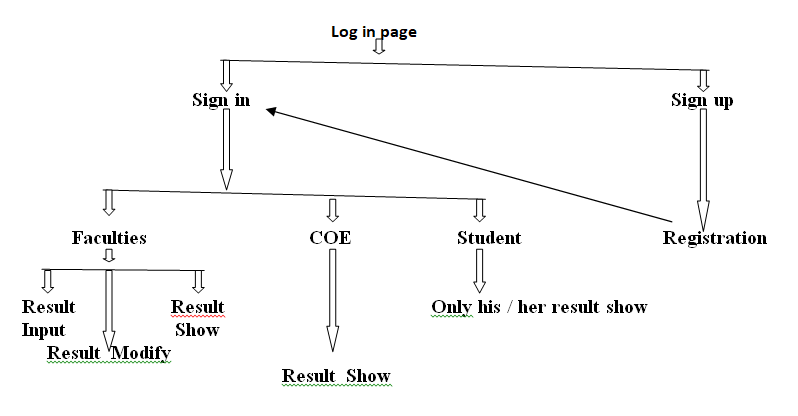
\includegraphics[width=.9\textwidth]{Metho.png}

\end{figure}

\label{oject}
Access point :

\begin{figure}[h!]
\centering
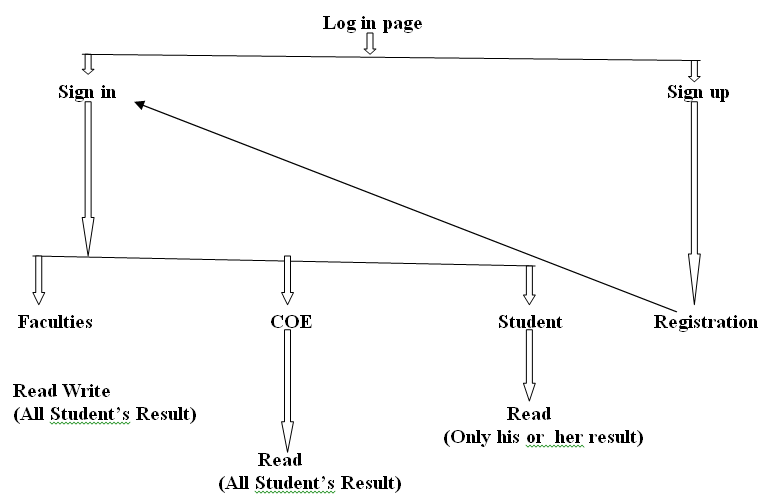
\includegraphics[width=.9\textwidth]{Access.png}

\end{figure}

\vspace{10cm}

\section{Platform and Tools}\label{oject}

Here, we use MYSQL for data base. HTML, CSS, JAVA SCRIPT for frontend design and LARAVEL for framework.


\section{Outline}\label{oject}

There will be two option in our Log in page. One option is Sign in and Another one is Sign up. There will be Sign in and Sign up for Faculties, COE and Students. Different access for Faculties, COE and Students will also be available here.

\section{References}\label{oject}
I.	Udemy Course Tutorial about HTML,CSS,JAVA SCRIPT,LARAVEL \\
II.	University course material: MYSQL \\
III. \url{https://www.youtube.com/results?search_query=coder+foundation} \\
IV. \url{https://www.youtube.com/channel/UCzmI_aDsHbBXPZzabrsM7sA}

\vspace{10cm}
\label{oject}
This proposal is approved by,\\ \\


\hspace{300pt} \line(1,0){170}	

\hspace{325pt} Supervisor Signature\\



\end{titlepage}
\end{document}



